\chapter{Simulador Metagenómico PyMetaSeem}

Uno de los principales desafíos en metagenómica es evaluar la calidad del ensamblaje y la correcta asignación taxonómica de los datos. Para ello, es fundamental contar con datos metagenómicos de referencia de alta calidad, que incluyan un sistema de clasificación riguroso y validado. Estos datos permiten evaluar el desempeño de las herramientas de ensamblaje y clasificación taxonómica.\\

En respuesta a esta necesidad, se han desarrollado diversos simuladores de datos metagenómicos. Sin embargo, como se analiza en este capítulo, la mayoría de estos simuladores presentan limitaciones que dificultan su uso. Entre los principales problemas se encuentran la complejidad en la instalación y configuración, la falta de flexibilidad en la parametrización de los datos simulados y la ausencia de modelos realistas que reflejen con precisión la diversidad y complejidad de las comunidades microbianas naturales.\\

Ante este panorama, se justifica la creación de un nuevo simulador de datos metagenómicos que supere estas dificultades y brinde una herramienta más efectiva para la evaluación de software en este campo. Un simulador ideal debe permitir la generación de reads metagenómicos con parámetros ajustables, garantizar la reproducibilidad de los experimentos, incluir modelos de error realistas y ofrecer una interfaz accesible para facilitar su uso en distintos contextos de investigación.\\

\begin{figure}[H]
\centering
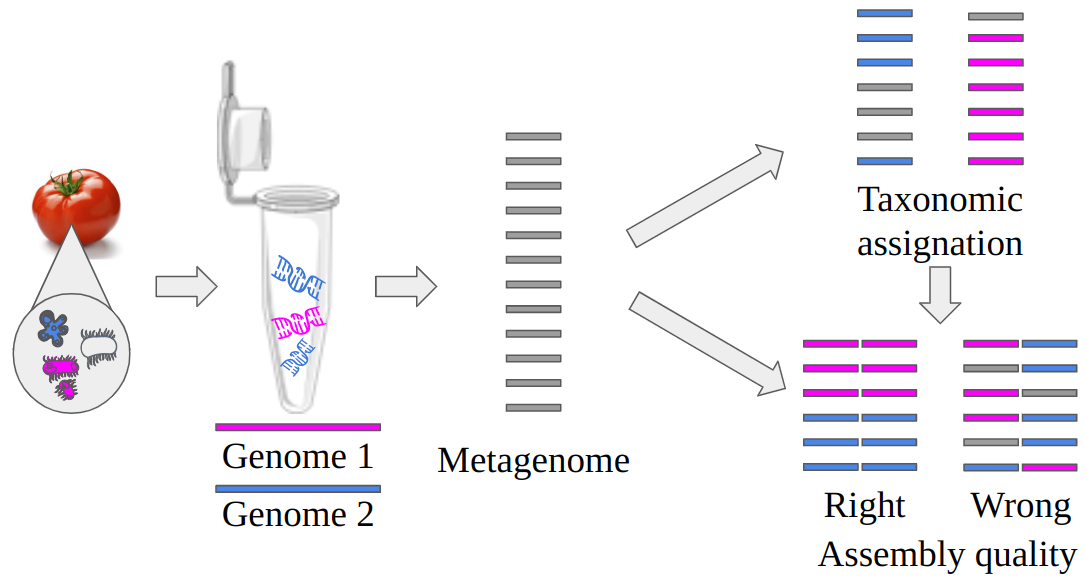
\includegraphics[width=\textwidth]{Img/cap4/problem.png}
\caption{ggg }
\end{figure}

En este capítulo se presenta el desarrollo de PyMetaSeem, un simulador diseñado desde cero para abordar estas limitaciones. Su implementación busca proporcionar una solución escalable, reproducible y de fácil acceso para la comunidad científica. Se detallan los principios de su diseño, su estructura funcional y sus ventajas frente a los simuladores existentes, demostrando su potencial como herramienta clave en la validación de metodologías de análisis metagenómico.\\


\section{PyMetaSeem: Un simulador de datos metagenómicos basado en secuencias genómicas}

El análisis metagenómico requiere herramientas precisas para la clasificación taxonómica y el ensamblaje de secuencias. Sin embargo, la evaluación de estas herramientas depende en gran medida de la disponibilidad de datos metagenómicos de referencia de alta calidad. En respuesta a esta necesidad, se ha desarrollado PyMetaSeem, un algoritmo diseñado desde cero para la simulación de datos metagenómicos a partir de secuencias genómicas.\\

PyMetaSeem permite la generación de reads metagenómicos sintéticos mediante el procesamiento de secuencias genómicas reales, proporcionando datos controlados y reproducibles para la evaluación de clasificadores taxonómicos y ensambladores de secuencias. A diferencia de otros simuladores como CAMISIM, que presentan dificultades en su instalación e implementación, PyMetaSeem ha sido desarrollado como un entorno Conda, garantizando escalabilidad, reproducibilidad y facilidad de uso. Su diseño modular y su código abierto facilitan su integración en diversos flujos de trabajo bioinformáticos, permitiendo su aplicación en múltiples estudios metagenómicos.\\

El algoritmo está compuesto por diversas funciones que permiten la generación de datos metagenómicos sintéticos de manera estructurada y eficiente. Inicialmente, recibe un conjunto de archivos en formato FASTA que contienen distintos genomas. La configuración de los parámetros de simulación puede realizarse manualmente o mediante un archivo de texto que especifica el número de reads por genoma, permitiendo la definición de un perfil taxonómico detallado y adaptable a distintos escenarios experimentales.\\

\begin{figure}[H]
\centering
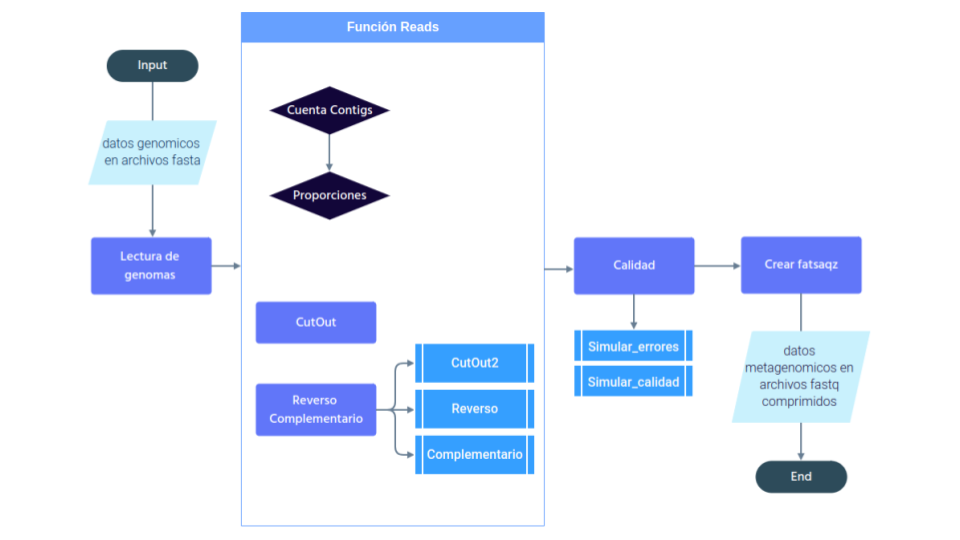
\includegraphics[width=\textwidth]{Img/cap4/diagrams_de_flujo.png}
\caption{Diagrama de Flujo PyMetaSeem}
\end{figure}

Una de las funciones clave de PyMetaSeem es la lectura y procesamiento de los archivos FASTA, los cuales son convertidos en una estructura de diccionario donde cada secuencia de nucleótidos se almacena como valor y su identificador como clave. Esta representación facilita la manipulación eficiente de los datos dentro del entorno de Python y optimiza el acceso a las secuencias genómicas para su posterior procesamiento.\\

A partir de los genomas almacenados en diccionarios, PyMetaSeem implementa funciones para determinar la longitud y la proporción de los reads a generar, teniendo en cuenta el tamaño original de los contigs. Posteriormente, se lleva a cabo la extracción de reads de manera aleatoria, garantizando que la longitud y distribución de los fragmentos reflejen con precisión la composición genómica original. Además, el algoritmo simula la calidad de los reads generados, incorporando modelos de error realistas que permiten una representación más precisa de los datos metagenómicos experimentales.\\

Finalmente, PyMetaSeem genera un archivo en formato FASTQ, que contiene las secuencias de reads metagenómicos junto con sus respectivas calidades de lectura. Este archivo puede ser utilizado en diferentes herramientas de ensamblaje y clasificación taxonómica, facilitando la evaluación de la precisión y eficiencia de estos métodos.\\


\subsection{Simulaciones}

%\begin{figure}[H]
%\centering
%
\includegraphics[width=\textwidth]{Img/cap2/clavibacter.png}
%\caption{Clavibacter}
%\end{figure}

\subsection{Comparaciones}


\section{Comparación taxonomica}

\section{Generalizando el N50, nuevas métricas para ensamblados de metagenoma}

En cuanto a la calidad de los ensamblajes, evaluamos la pertinencia de aplicar la métrica genómica N50 a los datos metagenómicos.  \\
(Videvall, 2017)  \\

Se trata de una medida utilizada para evaluar la contigüidad y la calidad del ensamblaje de un genoma. Los contigs de un ensamblaje se ordenan por tamaño y se suman, empezando por el mayor. Se toma el tamaño del contig que hace que el total sea mayor o igual al 50\% del tamaño del genoma.  \\


%\begin{figure}[H]
%\centering
%
\includegraphics[width=\textwidth]{Img/cap2/N50_es.png}
%\caption{N50 }
%\end{figure}

N50 es una medida de calidad de secuencias genómicas (Miller et al., 2010; Videvall, 2017) (“metagenómica”), la cual se mide ordenando la totalidad de las secuencias de mayor a menor longitud, y sumando todas las longitudes hasta llegar al 50\% del total de la suma; la longitud de la secuencia que esté en este 50\% será la medida N50.  \\

Una medida típica para evaluar el éxito del ensamblaje es la medida N50, que equivale a la longitud del scaffold (o contig) que se solapa con el punto medio de la concatenación de scaffolds (contigs) por orden de longitud. Mäkinen, V., Salmela, L. \& Ylinen, J. Métrica de ensamblaje N50 normalizada mediante encadenamiento colineal restringido por espacios. BMC Bioinformática 13 , 255 (2012). https://doi.org/10.1186/1471-2105-13-255   \\

L50 es una medida de calidad de secuencias genómicas\\
